% -*- TeX -*- -*- UK -*-
% ----------------------------------------------------------------
% arXiv Paper ************************************************
%
% Subhaneil Lahiri's template
%
% Before submitting:
%    Comment out hyperref
%    Comment out showkeys
%    Replace \input{mydefs.tex} with its contents
%       or include mydefs.tex in zip/tar file
%    Replace \input{newsymb.tex} with its contents
%       or include newsymb.tex in zip/tar file
%    Put this file, the .bbl file, any picture or
%       other additional files and natbib.sty
%       file in a zip/tar file
%
% **** -----------------------------------------------------------
\documentclass[12pt]{article}
%Preamble:
\usepackage{a4wide}
\input{sl_preamble.tex}
\input{sl_graphics_preamble.tex}
\graphicspath{{"Figures/"}}
%
\usepackage{array}
\newcounter{tablerow}
\newcommand{\tablerowautorefname}{row}
\newenvironment{tabularn}[1]{\setcounter{tablerow}{0}\begin{tabular}{#1>{\refstepcounter{tablerow}}l}}{\end{tabular}}
%\usepackage{etoolbox}
%\AtBeginEnvironment{tabular}{\setcounter{tablerow}{0}}
%
% >> Only for drafts! <<
\usepackage[notref,notcite]{showkeys}
% ----------------------------------------------------------------
%\numberwithin{equation}{section}
%\renewcommand{\baselinestretch}{1.5}
% ----------------------------------------------------------------
% New commands etc.
\input{sl_definitions.tex}
\input{sl_symbols.tex}
%matrices
\newcommand{\inv}{^{-1}}
\newcommand{\dg}{^\mathrm{dg}}
\newcommand{\trans}{^\mathrm{T}}
\newcommand{\I}{\mathbf{I}}
%vec of ones
\newcommand{\onev}{\mathbf{e}}
%mat of ones
\newcommand{\onem}{\mathbf{E}}
%Markov matrix
\newcommand{\MM}{\mathbf{Q}}
%equilibrium distribution
\newcommand{\pr}{\mathbf{p}}
\newcommand{\eq}{\pr^\infty}
%first passage times
\newcommand{\fpt}{\mathbf{T}}
%off-diag first passage times
\newcommand{\fptb}{\overline{\fpt}}
%fundamental matrix
\newcommand{\fund}{\mathbf{Z}}
%other symbols
\newcommand{\Pb}{\mathbf{P}}
\newcommand{\D}{\mathbf{D}}
\newcommand{\pib}{\boldsymbol{\pi}}
\newcommand{\Lb}{\boldsymbol{\Lambda}}
\newcommand{\w}{\mathbf{w}}
\newcommand{\W}{\mathbf{W}}
\newcommand{\frg}{\W^\mathrm{F}}
\newcommand{\M}{\mathbf{M}}
\newcommand{\F}{\boldsymbol{\Phi}}
\DeclareMathOperator{\SNR}{SNR}
\newcommand{\CS}{\mathcal{S}}
\newcommand{\CA}{\mathcal{A}}
\newcommand{\CB}{\mathcal{B}}
\newcommand{\comp}{^\mathrm{c}}
\newcommand{\pot}{^{\text{pot}}}
\newcommand{\dep}{^{\text{dep}}}
\newcommand{\potdep}{^{\text{pot/dep}}}
\newcommand{\norm}{_0}
\newcommand{\inc}{_{\text{inc}}}
\newcommand{\dec}{_{\text{dec}}}
\newcommand{\incdec}{_{\text{inc/dec}}}
\newcommand{\wt}{_{\text{WT}}}
\newcommand{\ko}{_{\text{D$^\mathrm{b}$K$^\mathrm{b}$-/-}}}
\newcommand{\KO}{D$^\mathrm{b}$K$^\mathrm{b}$-/-}
\newcommand{\tpre}{t_{\text{pre}}}
\newcommand{\ttrain}{t_{\text{train}}}
\newcommand{\lmax}{_{\text{max}}}
\newcommand{\lmin}{_{\text{min}}}
% ----------------------------------------------------------------
%
%%%%%%%%%%%%%%%%%%%%%%%%%%%%%%%%%%%%%%%%%%%%%%%%%%%%%%%%%%%%%%%%%%%%%%%%%%
% Title info:
\title{Models of VOR learning in MHC knockout mice}
%
% Author List:
%
\author{Subhaneil Lahiri
%
}

\begin{document}

\maketitle


%%%%%%%%%%%%%%%%%%%%%%%%%%%%%%%%%%%%%%%%%%%%%%%%%%%%%%%%%%%%%%%%%%%%%%%%%%


\begin{abstract}
  We see if we can model VOR gain increase and decrease learning in mice with a knockout in MHC as well as wild-type.
\end{abstract}

\tableofcontents

%%%%%%%%%%%%%%%%%%%%%%%%%%%%%%%%%%%%%%%%%%%%%%%%%%%%%%%%%%%%%%%%%%%%%%%%%%
% Beginning of Article:
%%%%%%%%%%%%%%%%%%%%%%%%%%%%%%%%%%%%%%%%%%%%%%%%%%%%%%%%%%%%%%%%%%%%%%%%%%

\section{Introduction and summary}\label{sec:intro}

We will see if we can capture the essential features of VOR gain-increase learning in wild type and MHC \KO\ mutants and wild-type, with and without gain-decrease pre-training.
We will try to do this using models of complex synapses, such as the cascade model \cite{Fusi2005cascade} or the multistate model \cite{amit1994learning,Fusi2007multistate}.
We will also construct a new model in \autoref{sec:pooledmodel} that incorporates the idea that biasing the synapses in one direction could deplete some resource, thereby impairing further plasticity in the same direction in nearby synapses.

These models all assume independent, statistically identical synapses.
This has the benefit of freeing us from modelling the neurons and their networks, allowing us to focus on the synapses themselves.
However, we will lose certain aspects of real synapses.
For example, during gain-increase learning, certain synapses will be potentiated more often and others will be depressed more often.
In these models, however, synaptic identity is not kept track of, so training can only be described by changing the overall levels of potentiation and depression.

As the MHC \KO\ mutation lowers the threshold for LTD, we will model these mice by increasing the probabilities for internal synaptic transitions associated with depression, whilst leaving potentiation unchanged.

We will be parsimonious in our modelling.
We will assume that the wild-type has a symmetry between potentiation and depression and we will treat gain-increase and decrease training in a symmetric way.
We will also assume that the relative rates of potentiation/depression in the mutant and wild-type are the same and that the overall rate of plasticity events is the same in all situations.
None of these assumptions are necessary or justified experimentally (although \cite{Fusi2007multistate} notes that imbalance between potentiation and depression can drastically impair memory).
They do reduce the number of adjustable parameters we have, simplifying searches for good models.
Presumably, relaxing these assumptions and enlarging the parameter space would allow for a better fit to data, but the number of parameters would start to look large compared to the number of features we're trying to match.

If we imagine something like an LN model for the Purkinje cell, the output would depend on some linear combination of the synaptic weights (weighted by the activities of the corresponding parallel fibres).
If we're not keeping track of synaptic identity, the most natural linear combination to use would be an equal sum of them all.
Thus we will quantify learning by the change in the mean synaptic weight.

The output of the Purkinje cell, and the behavioural output of the animal, will depend on this quantity in some complicated nonlinear way.
Modelling this is far beyond the scope of this work.
Instead we will look at more qualitative features, asking whether learning is slower or faster in some situation compared to another.

Within the parameter range explored, we will see that synaptic complexity is essential.
The simple two-state model always shows enhanced learning in the mutant (see \autoref{fig:binary}), in contradiction with experiment.
It seems that the enhanced depressing transition more than compensates for saturation effects.

On the other hand, the cascade, multistate and pooled resource models all have parameter ranges where the mutant has impaired learning without pre-training (see \autoref{fig:cascade_short}, \autoref{fig:cascade_long}, \autoref{fig:multistate_weak}, \autoref{fig:multistate_strong} and \autoref{fig:pooled_scarce}).
We have found parameter ranges where the reverse happens for the multistate (see discussion below \eqref{eq:multiKOnopre}) and the pooled resource model (see \autoref{fig:pooled_plenty}).
These rely on properties of the mutation, so it would be difficult to explore with further experiments.

All of these models show pre-training enhancing learning for the mutant, as expected.
It is harder to find regimes where pre-training impairs learning for the wild-type.
In the cascade model, this required a much longer duration for pe-training (see \autoref{fig:cascade_long}).
In the multistate model, this required stronger training, which resulted in gain-decrease learning being faster for the mutant then wild-type (see \autoref{fig:multistate_strong}), unlike what is seen experimentally.
It is possible that these features could be improved by lessening the symmetry between gain-increase and decrease or potentiation and depression, or by allowing the rate of plasticity events to vary.
For the pooled resource model, we haven't found any parameter regime where pre-training impairs learning for the wild-type, and we discuss why it seems unlikely in \autoref{sec:pooled}.

There seems to be two take home messages.
First, impaired learning without pre-training in the mutant requires synaptic complexity, as it is not seen in the simple two-state model.
Second, impaired learning with pre-training in the wild-type requires a form of metaplasticity where repeated potentiation makes subsequent depression less likely.
This is a feature of the cascade model and our version of the multistate model, but not the pooled resource model.


\section{The setup}\label{sec:setup}


\subsection{Models of synapses}\label{sec:synapse}

We make the following assumptions:
\begin{itemize}
  \item There are $N$ identical synapses with $M$ internal functional states.
  \item The states of different synapses are independent of each other.
  \item The synapses that are eligible for plasticity are chosen randomly.
  \item The potentiating/depressing plasticity event timings are distributed as Poisson processes with rates $rf\potdep$, where $f\pot+f\dep=1$.
      In other words, $r$ is the total rate of plasticity events per synapse and $f\potdep$ are the fraction of these events that are potentiating/depressing.
  \item Potentiation and depression are described by Markov processes with transition probabilities $\M\potdep$.
  \item The synaptic weights of the internal states are given by the column vector $\w$. This can only take two values that we can call $\pm1$, except for the pooled resource model that we will discuss in \autoref{sec:pooledmodel} and \autoref{sec:pooled}.
\end{itemize}

The independence and identicalness of synapses means that the state of the system can be completely described by the probability distribution of the internal states, the row vector $\pr(t)$.

The evolution of this probability is described by a forgetting matrix, $\frg$:
%
\begin{equation}\label{eq:evolve}
  \diff{\pr(t)}{t} = r\pr(t)\frg,
  \qquad
  \frg = f\pot\M\pot+f\dep\M\dep-\I,
\end{equation}
where $\I$ is the identity matrix.
%
Eventually, this will settle into the equilibrium distribution:
%
\begin{equation}\label{eq:eqprob}
  \eq\frg=0.
\end{equation}
%



With only two possible synaptic weights, the distribution of synaptic weights is completely described by the mean, $\pr(t)\w$.


\subsection{Model of VOR learning experiment}\label{sec:learning}

Training the animal will not change the internal dynamics of a synapse under potentiation or depression.
It will change the environment, will lead to a change in how often potentiation and depression occur.
It could be manifested in a change in which synapses are potentiated/depressed, but this could not be captured in this type of model.
We will model this by changing $f\potdep$, leaving $r$ and $\M\potdep$ unchanged.

The untrained case will be described by $f\pot=f\pot\norm$.
Gain-increase training  will be described by $f\pot=f\pot\inc<f\pot\norm$, and
gain-decrease training  will be described by $f\pot=f\pot\dec>f\pot\norm$. Note that the forgetting matrix \eqref{eq:evolve} and the equilibrium distribution \eqref{eq:eqprob} depend on $f\pot$, which we will indicate with subscripts.

Before training, the synaptic distribution will in equilibrium with $f\pot\norm$.
During gain-increase training, it will evolve according to \eqref{eq:evolve} with $f\pot\inc$:
%
\begin{equation}\label{eq:nopre}
  \pr(t) = \eq\norm \exp\prn{rt\frg\inc}.
\end{equation}
%
On the other hand, if the gain-increase training follows gain-decrease pre-training for some time period, $\tpre$:
%
\begin{equation}\label{eq:withpre}
  \pr(t) = \eq\norm \exp\prn{r\tpre\frg\dec} \exp\prn{r(t-\tpre)\frg\inc}.
\end{equation}
%

We will describe the effect of training by the decrease in mean synaptic weight:
%
\begin{equation}\label{eq:learning}
  L(t) = \prn{\pr(0)-\pr(t)}\w.
\end{equation}
%
The behavioural output (VOR gain) will be some non-linear function of the synaptic weights, so the best we can hope for is to reproduce qualitative features of the experiment.

The MHC mutant has a lower threshold for depression.
We can model this by changing $\W\dep\wt$ to $\W\dep\ko$, which should have larger matrix elements.

QUESTION: Should $f\pot\wt=f\pot\ko$?

If they are equal, this would change the mean synaptic weight in equilibrium.
This seems like it could affect the ability of the network to perform its function, whereas, in reality, the wild-type and mutant have the same baseline performance.
In any case, if the synaptic weights are different, the electrical activity will be different, and there will be no reason to expect the same statistics for potentiation or depression.
In setting $f\pot\wt=f\pot\ko$, we are assuming that the rest of the brain compensates for the difference in synaptic weights somehow.

On the other hand, one could imagine adjusting $f\pot\wt$ and $f\pot\ko$ so that $\eq\wt\w = \eq\ko\w$.
But, now that the synaptic weights are the same, the electrical activity will be the same, and there will be no reason to expect different statistics for potentiation or depression.
If we did this for the multistate or two-state models, we'd remove all differences between the wild-type and \KO\ mutant, so we won't.

We are also assuming that the relation between VOR gain and mean synaptic weight is the same for mutant ant wild-type, except for a linear offset to compensate for the difference in equlibrium weights mentioned above.


\section{Simulations}\label{sec:sims}

\subsection{Models and parameters}

We will look at three different models, the cascade model (see \cite{Fusi2005cascade} and \autoref{fig:models}\ref{fig:cascade_model}), the multistate model\footnote{The version of the multistate model that we'll study is slightly different than the original definition. We will only allow the synaptic weight to take two values, whereas it originally varied linearly across the states. } (see \cite{amit1994learning,Fusi2007multistate} and \autoref{fig:models}\ref{fig:multistate_model}) and the two-state model (which can be thought of as a special case of the previous two, see \autoref{fig:models}\ref{fig:binary_model}).
We will also look at a new, pooled resource model that we will define below in \autoref{sec:pooledmodel}.

For the cascade model, we will use the same value for the parameter $x$ (which controls the decay of transition rates, see \cite{Fusi2005cascade}) for potentiation and depression in the wild-type as well as potentiation in the \KO\ mutant.
We will use a larger value for $x$ for depression in the \KO\ mutant.

For the multistate and two state models, we will use the same value for the transition probabilities, $q$, for potentiation and depression in the wild-type as well as potentiation in the \KO\ mutant.
We will use a larger value for $q$ for depression in the \KO\ mutant.

In each case, we set $f\pot\norm=\half$, $f\pot\inc=f\pot\norm+\Delta f$ and $f\pot\dec=f\pot\norm-\Delta f$.
We use the same values for wild-type and mutant and treat gain-increase and decrease symmetrically.
The values of all these parameters are listed in \autoref{tab:params}.

\begin{figure}
 \begin{center}
 \begin{myenuma}
  \item\aligntop{\includegraphics[height=2cm]{cascade.svg}}\label{fig:cascade_model}\hspace{0.5cm}
  \item\aligntop{\includegraphics[height=1.7cm]{multistate.svg}}\label{fig:multistate_model}\hspace{0.5cm}
  \item\aligntop{\includegraphics[height=1.7cm]{binary.svg}}\label{fig:binary_model}
 \end{myenuma}
 \end{center}
  \caption{Transition probabilities for different models.
  (\ref{fig:cascade_model}) In the cascade model, the transition probabilities decay geometrically with a parameter $x$ (see \cite{Fusi2005cascade}).
  (\ref{fig:multistate_model}) In the multistate model the transition probabilities for potentiation/depression are all equal and it is parameterised by these two values.
  (\ref{fig:binary_model}) The two-state model is parameterised by the two transition probailities.} \label{fig:models}
\end{figure}

\begin{table}
 \begin{center}
  \begin{tabularn}{|l|c|c|c|c|c|c|}
    \cline{1-7}
    % after \\: \hline or \cline{col1-col2} \cline{col3-col4} ...
    Model & \# states & pot,WT dep & \KO\ dep & $\Delta f$ & $r\ttrain$ & $r\tpre$ \\
    \cline{1-7}
    Cascade    & 10 & $x=0.25$ & $x=0.33$ & -0.3 & 50 & 50  &\label{tr:cascade_short} \\
    Cascade    & 10 & $x=0.25$ & $x=0.33$ & -0.3 & 50 & 150 &\label{tr:cascade_long} \\
    Multistate & 10 & $q=0.6$  & $q=0.8$  & -0.1 & 50 & 50  &\label{tr:multistate_weak} \\
    Multistate & 10 & $q=0.6$  & $q=0.8$  & -0.4 & 20 & 20  & \label{tr:multistate_strong} \\
    Two-state  & 2  & $q=0.4$  & $q=0.8$  & -0.1 & 5  & 5   &\label{tr:binary} \\
    Pooled     & 10 & $q\in[0.3,0.4]$  & $q\in[0.6,0.8]$
                                          & -0.1 & 70 & 70 &\label{tr:pooled_plenty}\\
    Pooled     & 10 & $q\in[0.1,0.4]$  & $q\in[0.2,0.8]$
                                          & -0.1 & 70 & 70 &\label{tr:pooled_scarce}\\
    \cline{1-7}
%   \hline
%    % after \\: \hline or \cline{col1-col2} \cline{col3-col4} ...
%    & Model & \# states & pot,WT dep & \KO\ dep & $\Delta f$ & $r\ttrain$ & $r\tpre$ \\
%    \cline{1-7}
%    \label{tr:cascade_short}&
%    Cascade    & 10 & $x=0.25$ & $x=0.33$ & -0.3 & 50 & 50   \\
%    \label{tr:cascade_long}&
%    Cascade    & 10 & $x=0.25$ & $x=0.33$ & -0.3 & 50 & 150  \\
%    \label{tr:multistate_weak}&
%    Multistate & 10 & $q=0.6$  & $q=0.8$  & -0.1 & 50 & 50   \\
%    \label{tr:multistate_strong}&
%    Multistate & 10 & $q=0.6$  & $q=0.8$  & -0.4 & 20 & 20   \\
%    \label{tr:binary}&
%    Two-state  & 2  & $q=0.4$  & $q=0.8$  & -0.1 & 5  & 5    \\
%    \label{tr:pooled_plenty}&
%    Pooled     & 10 & $q\in[0.3,0.4]$  & $q\in[0.6,0.8]$
%                                          & -0.1 & 70 & 70 \\
%    \label{tr:pooled_scarce}&
%    Pooled     & 10 & $q\in[0.1,0.4]$  & $q\in[0.2,0.8]$
%                                          & -0.1 & 70 & 70 \\
%    \cline{1-7}
  \end{tabularn}
 \end{center}
  \caption{Parameters used in simulations.} \label{tab:params}
\end{table}

\subsubsection{Pooled resource model}\label{sec:pooledmodel}

Suppose that there is some resource required for potentiation/depression that is shared between $P$ synapses and is depleted as more synapses are potentiated/depressed.
We can avoid going beyond the independent synapse model by modelling this pool of synapse as a single compound synapse.

We will model the individual synapses with the two-state model.
Let $i$ be the number of them that are potentiated.
We will model the effect of resource depletion linearly with the potentiation/depression probabilities for the individual synapses:
%
\begin{equation}\label{eq:depletion}
  \begin{aligned}
    q\pot &= \frac{(P-i-1)q\lmax + i\,q\lmin}{P-1}, \qquad
    q\dep &= \frac{(i-1)q\lmax + (P-i)q\lmin}{P-1}.
  \end{aligned}
\end{equation}
%
At each plasticity event for the compound synapse, one of the individual synapses will be chosen randomly for update.
This effectively reduces the transition probabilities by $1/P$.

This compound synapse would seem to have $2^P$ internal states.
However, we need only keep track of the number of potentiated synapses, not their identity, leaving $M=P+1$ states.
The transition network topology will then have a multistate toplogy (see \autoref{fig:models}\ref{fig:multistate_model}) but the transition probabilities will no longer be uniform and the weight of the compound synapse is the mean of its constituent synapses:
%
\begin{equation}\label{eq:pooledweight}
  \w_i = \frac{2i}{P}-1.
\end{equation}
%


The Markov process is lumpable \wrt this partition of states (see \cite[\S6.3]{kemeny1960finite} for the discrete time version and \cite{burke1958markovian,Ball1993Lumpability} for continuous time).
The transition probabilities between lumps $i$ and $j$ is computed by choosing one state from lump $i$ and summing the transition probabilities to all states in lump $j$.
The result must be the same for all states in lump $i$.

For any state in lump $i$, there are $P-i$ synapses that can be potentiated to go to lump $i+1$.
Each of these transition probabilities is $q\pot/P$.
Similarly, there are $i$ synapses that can be depressed to go to lump $i-1$.
Each of these transition probabilities is $q\dep/P$.
Thus:
%
\begin{equation}\label{eq:pooledpotdep}
  \begin{aligned}
    \M\pot_{ii+1} &=  \brk{\frac{(P-i-1)q\lmax + i\,q\lmin}{P-1}} \frac{P-i}{P}, \\
    \M\dep_{ii-1} &=  \brk{\frac{(i-1)q\lmax + (P-i)q\lmin}{P-1}} \frac{i}{P},
  \end{aligned}
\end{equation}
%
with all other off-diagonal elements equal to zero.
The diagonal elements are chosen so that the rows sum to one.

This model is parameterised by the range of values, $q\in[q\lmin,q\lmax]$, for potentiation and depression.
We will use the same values for potentiation and depression in the wild-type as well as potentiation in the \KO\ mutant.
We will use larger values for depression in the \KO\ mutant.


\subsection{Results}\label{sec:results}

The features of the actual experiments that we'd like to capture are:
\begin{itemize}
  \item Without pre-training, gain-increase learning is significantly faster in the wild-type than in the mutant.
  \item Gain-decrease pre-training is slightly faster in the wild-type, but not significantly so.
  \item After pre-training, gain-increase learning is significantly faster in the mutant than in the wild-type.
  \item For the wild-type, gain-increase learning is significantly faster without pre-training than with it.
  \item For the mutant, gain-increase learning is significantly faster with pre-training than without it.
\end{itemize}

We will try to gain some analytic insight to some of these models by looking at the slope of the learning curve at the start of gain-increase training.
This is proportional to the net-flux between the $\w=+1$ states and the $\w=-1$ states, measuring using the transition probabilities for gain-increase but the equilibrium distribution for either untrained or gain-decrease, assuming that pre-training lasts long enough to reach the equilibrium distribution for gain-decrease.


\newcommand{\resultsfig}[2]{\begin{figure}
 \begin{center}
 \begin{myenuma}
  \item\aligntop{\includegraphics[width=7cm]{#1_learn.eps}}\label{fig:#1_learn}
  \item\aligntop{\includegraphics[width=7cm]{#1_learnS.eps}}\label{fig:#1_learnS}
  \item\label{fig:#1_eq}\begin{myenumi}
                    \item\aligntop{\includegraphics[width=7cm]{#1_eq_WT.eps}}\label{fig:#1_eq_WT}
                    \item\aligntop{\includegraphics[width=7cm]{#1_eq_KO.eps}}\label{fig:#1_eq_KO}
                  \end{myenumi}
  \item\label{fig:#1_pr}\begin{myenumi}
                    \item\aligntop{\includegraphics[width=3cm]{#1_pr_WT_nopre.eps}}\label{fig:#1_pr_WT_nopre}
                    \item\aligntop{\includegraphics[width=3cm]{#1_pr_WT_pre.eps}}\label{fig:#1_pr_WT_pre}
                    \item\aligntop{\includegraphics[width=3cm]{#1_pr_KO_nopre.eps}}\label{fig:#1_pr_KO_nopre}
                    \item\aligntop{\includegraphics[width=3cm]{#1_pr_KO_pre.eps}}\label{fig:#1_pr_KO_pre}
                  \end{myenumi}
 \end{myenuma}
 \end{center}
  \caption[#2]{#2.
  Other parameters can be found in \autoref{tr:#1} of \autoref{tab:params}.
  Time is measured in units of $1/r$, the mean time between plasticity events.
  (\ref{fig:#1_learn}) Learning curves for wild-type and \KO\ mutant with and without pre-training.
  (\ref{fig:#1_learnS}) Learning curves restricted to gain-increase training.
  (\ref{fig:#1_eq}) Equilibrium distributions without training or with gain-increase/decrease training for (\ref{fig:#1_eq_WT}) wild-type and (\ref{fig:#1_eq_KO}) \KO\ mutant.
  (\ref{fig:#1_pr}) Evolution of probability distributions for (\ref{fig:#1_pr_WT_nopre}\ref{fig:#1_pr_WT_pre}) wild-type and  (\ref{fig:#1_pr_KO_nopre}\ref{fig:#1_pr_KO_pre}) \KO\ mutant without (\ref{fig:#1_pr_WT_nopre},\ref{fig:#1_pr_KO_nopre}) and with (\ref{fig:#1_pr_WT_pre},\ref{fig:#1_pr_KO_pre}) pre-training. } \label{fig:#1}
\end{figure}}



\subsubsection{Cascade model}\label{sec:cascade}

\resultsfig{cascade_short}{Simulation results for cascade model with short pre-training ($rt_\text{pre}=50$)}

\resultsfig{cascade_long}{Simulation results for cascade model with long pre-training ($rt_\text{pre}=150$)}



The results of simulations of the cascade model can be seen in \autoref{fig:cascade_short} and \autoref{fig:cascade_long}.

In both of these, we see that the mutant is slower than wild-type without pre-training but faster with it.
This seems to be due to the fact that, without pre-training, very few synapses will be available for depression as most of them are already depressed (\autoref{fig:cascade_short}\ref{fig:cascade_short_eq}\ref{fig:cascade_short_eq_KO} and \ref{fig:cascade_short_pr}\ref{fig:cascade_short_pr_KO_nopre}).
With pre-training, some of them will now be potentiated (\autoref{fig:cascade_short}\ref{fig:cascade_short_eq}\ref{fig:cascade_short_eq_KO} and \ref{fig:cascade_short_pr}\ref{fig:cascade_short_pr_KO_pre}), and the enhanced depression can speed up learning.

With shorter pre-training, we see that it speeds up learning in both wild-type and mutant (see \autoref{fig:cascade_short}\ref{fig:cascade_short_learnS}), whereas experimentally this only happens for the mutant.
This is due to the fact that pre-training results in more synapses being potentiated, and thus ready for depression, but does not push them far enough down the cascade for the lower transition probabilities to slow down learning.

We can see from \autoref{fig:cascade_long}\ref{fig:cascade_long_learnS} that longer pre-training pushes the synapses further down the cascade, slow in down learning for the wild-type.
This effect is weaker for the mutant, as the equilibrium distribution is not as heavily concentrated at the end (see \autoref{fig:cascade_long}\ref{fig:cascade_long_eq}\ref{fig:cascade_long_eq_KO}).


\subsubsection{Multistate model}\label{sec:multistate}

\resultsfig{multistate_weak}{Simulation results for multistate model with weak training ($\Delta f=-0.1$)}

\resultsfig{multistate_strong}{Simulation results for multistate model with strong training ($\Delta f=-0.4$)}


The results of simulations of the multistate model can be seen in \autoref{fig:multistate_weak} and \autoref{fig:multistate_strong}.
However, we can get some insight into this model analytically.



Consider the general uniform multistate model.
Then the equilibrium distribution is given by
%
\begin{equation}\label{eq:mutltieq}
  \eq_i = \frac{1-\alpha}{1-\alpha^M}\,\alpha^{i-1},
  \qquad \text{where} \quad
  \alpha=\frac{f\pot q\pot}{f\dep q\dep}.
\end{equation}
%
If we take the limit $\alpha\rightarrow1$, this becomes $\frac{1}{M}$.

The net-flux from the $\w=+1$ states to the $\w=-1$ states is:
%
\begin{equation}\label{eq:multiflux}
  \Phi = \eq_{M/2+1}f'{}\dep q\dep - \eq_{M/2}f'{}\pot q\pot = \frac{1-\alpha}{1-\alpha^M}\,\alpha^{M/2-1}\prn{\alpha-\alpha'}f'{}\dep q\dep,
\end{equation}
%
where primed values correspond to the new value of $f\pot$.

First, consider the wild-type, for which $q\pot=q\dep=q$.
Without pre-training:
%
\begin{equation}\label{eq:multiWTnopre}
  \Phi = -\frac{2\Delta fq}{M},
\end{equation}
%
where it's worth remembering that $\Delta f<0$.
With pre-training:
%
\begin{equation}\label{eq:multiWTpre}
\begin{aligned}
  \Phi &= 16(\Delta f)^2q \, \frac{(1-2\Delta f)^{M/2-1} (1+2\Delta f)^{M/2-1}}
          {(1-2\Delta f)^M - (1+2\Delta f)^M} \\
       &= -\frac{4\Delta fq}{M} + \CO(\Delta f)^2.
\end{aligned}
\end{equation}
%
So, we see that pre-training will speed up learning when $\Delta f$ is small (in absolute value), as seen in \autoref{fig:multistate_weak}\ref{fig:multistate_weak_learnS}.
On the other hand, if $\Delta f$ is close to $-\half$, pre-training will initially slow down learning a lot, as seen in \autoref{fig:multistate_strong}\ref{fig:multistate_strong_learnS}.

Intuitively, the flux depends on the slope of the distribution at the centre of the chain (with an offset due to the difference between $f\pot$ and $f\dep$).
Pre-training has two effects: it produces a slope in the right direction (see \autoref{fig:multistate_weak}\ref{fig:multistate_weak_eq}), but it also reduces distribution at the centre (see \autoref{fig:multistate_strong}\ref{fig:multistate_strong_eq}).
For small $\Delta f$, the first effect is stronger and learning speeds up.
For larger $\Delta f$, the second effect wins and learning slows down.

Now, consider the mutant, for which $q\pot=\beta q\dep=q$, $\beta<1$.
Without pre-training:
%
\begin{equation}\label{eq:multiKOnopre}
  \Phi = -2\Delta f q\,\frac{(1-\beta)\beta^{M/2-1}}{1-\beta^M}.
\end{equation}
%
This will be smaller than \eqref{eq:multiWTnopre} if $\beta<\beta^*(M)$.
This function is plotted in \autoref{fig:multistate_star}\ref{fig:multistate_betastar}, where we can see that it approaches 1 rapidly as we increase $M$.

There are two effects here as well.
Smaller $\beta$ will increase the probability of crossing the centre of the chain, speeding up learning, but it will also concentrate probability at the ends of the chain, depleting the centre and slowing down learning.
The first effect goes like $1/\beta$, whereas the second goes like $\beta^{M/2}$ and will be more significant for smaller $\beta$ or in a longer chain.

With pre-training:
%
\begin{equation}\label{eq:multiKOpre}
\begin{aligned}
  \Phi &= -4\Delta f q \, \frac{(1-2\Delta f) - \beta(1+2\Delta f)}
          {(1-2\Delta f)^M - \beta^M(1+2\Delta f)^M}   \,
          \beta^{M/2-1}(1-2\Delta f)^{M/2-1} (1+2\Delta f)^{M/2-1} \\
       &= -4\Delta f q\,\frac{(1-\beta)\beta^{M/2-1}}{1-\beta^M} + \CO(\Delta f)^2.
\end{aligned}
\end{equation}
%
Once again, we see that pre-training will speed up learning when $\Delta f$ is small, whereas, if $\Delta f$ is close to $-\half$, pre-training will initially slow down learning.

Let us define $\Delta f^*(\beta,M)$ to be the value at which \eqref{eq:multiKOnopre} and \eqref{eq:multiKOpre} are equal.
As we would like pre-training to slow down learning in the wild-type but speed it up in the mutant, it would seem that we require $\Delta f^*(\beta,M) < \Delta f < \Delta f^*(1,M)$ (remembering once more that $\Delta f<0$ and that the wild-type corresponds to $\beta=1$).
However, as seen in \autoref{fig:multistate_star}\ref{fig:multistate_deltafstar}, $\Delta f^*(\beta,M) > \Delta f^*(1,M)$, which would make this impossible.

But, all is not lost.
This is only the initial, instantaneous rate of change.
Let's look at \autoref{fig:multistate_strong}\ref{fig:multistate_strong_learnS}, for which $\Delta f < \Delta f^*(1,M)$, so that pre-training initially slows down learning for both wild-type and mutant.
We see that the pre-trained curve can rapidly catch up with the un-pre-trained one, due to the mass of probability concentrated at the end of the chain (see \autoref{fig:multistate_strong}\ref{fig:multistate_strong_eq}) drifting to the centre.
This happens sooner for the mutant than the wild-type, due to the stronger depressing transitions.
This means that there is an intermediate range of time-scales over which pre-training does slow down learning in the wild-type but speed it up in the mutant.

In conclusion, if we choose $\beta<\beta^*(M)$, $\Delta f < \Delta f^*(1,M)$ and look at intermediate time-scales, we will see that the mutant learns slower than wild-type without pre-training, and that pre-training speeds up learning in the mutant but slows it down in the wild-type.
However, in this case pre-training proceeds much faster in the mutant than wild-type (see \autoref{fig:multistate_strong}\ref{fig:multistate_strong_learn}), which is \emph{not} seen in the experiment.



\begin{figure}
 \begin{center}
 \begin{myenuma}
  \item\aligntop{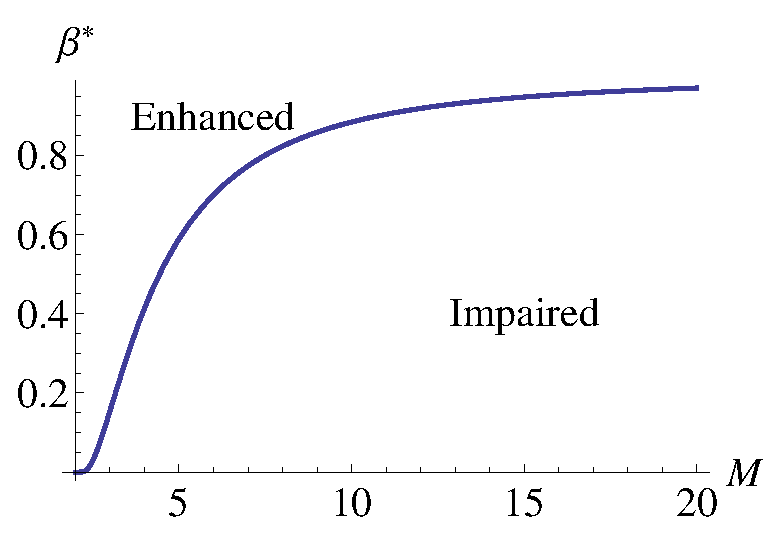
\includegraphics[width=7cm]{multistate_betastar.eps}}\label{fig:multistate_betastar}
  \item\aligntop{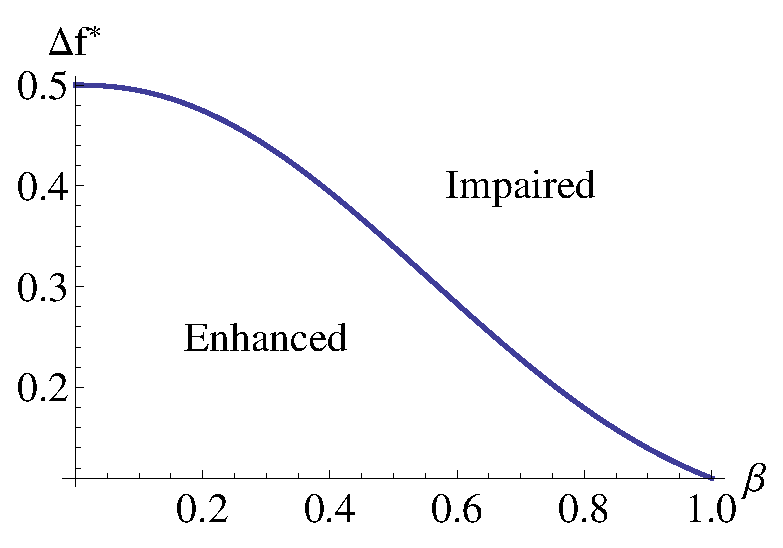
\includegraphics[width=7cm]{multistate_deltafstar.eps}}\label{fig:multistate_deltafstar}
 \end{myenuma}
 \end{center}
  \caption{The functions (\ref{fig:multistate_betastar}) $\beta^*(M)$ and (\ref{fig:multistate_deltafstar}) $\Delta f^*(\beta,M)$ for $M=10$.}\label{fig:multistate_star}
\end{figure}



\subsubsection{Two-state model}\label{sec:binary}


\resultsfig{binary}{Simulation results for two-state model}


The results of simulations of the two-state model can be seen in \autoref{fig:binary}.
However, this model can be solved exactly:
%
\begin{multline}\label{eq:binarysol}
  \eq = \frac{(f\dep q\dep, f\pot q\pot)}{\lambda},
  \qquad
  \pr(t) = \eq + (\pr(t)-\eq)\e^{-\lambda rt},\\
  \qquad \text{where} \quad
  \lambda = f\pot q\pot + f\dep q\dep.
\end{multline}
%
But it is easier to just substitute $M=2$ into the formulae in \autoref{sec:multistate}.
In this case, the initial rate of change encapsulates the whole solution, as there is only a single exponential decay.

First, consider the wild-type, for which $q\pot=q\dep=q$.
Without pre-training:
%
\begin{equation}\label{eq:binWTnopre}
  \Phi = -\Delta f q,
\end{equation}
%
where, again, it's worth remembering that $\Delta f<0$.
With pre-training:
%
\begin{equation}\label{eq:binWTpre}
\begin{aligned}
  \Phi &= -2\Delta f q.
\end{aligned}
\end{equation}
%
So, we see that pre-training will always speed up learning, unlike what is seen in the experiment.
This can be seen in \autoref{fig:binary}\ref{fig:binary_learnS}.

Now, consider the mutant, for which $q\pot=\beta q\dep=q$, $\beta<1$.
Without pre-training:
%
\begin{equation}\label{eq:binKOnopre}
  \Phi = -\frac{2\Delta f q}{1+\beta},
\end{equation}
%
which is always larger that \eqref{eq:binWTnopre}, unlike what is seen in the experiment.
This is also seen in \autoref{fig:binary}\ref{fig:binary_learn},\ref{fig:binary_learnS}.
As discussed below \eqref{eq:multiKOnopre}, the smaller values of has two effects.
Smaller $\beta$ will increase the probability of depression, speeding up learning, but it will also decrease the probability of being ready for depression, slowing down learning.
The second effect is much smaller for the very short chain considered here.

With pre-training:
%
\begin{equation}\label{eq:binKOpre}
\begin{aligned}
  \Phi &= -4\Delta f q \, \frac{(1-2\Delta f) - \beta(1+2\Delta f)}
          {(1-2\Delta f)^2 - \beta^2(1+2\Delta f)^2}.
\end{aligned}
\end{equation}
%
As we've already ruled out this model, we won't waste any time analysing this formula.


\subsubsection{Pooled resource model}\label{sec:pooled}


\resultsfig{pooled_plenty}{Simulation results for pooled resource model with light resource depletion ($q\lmin/q\lmax=0.75$)}

\resultsfig{pooled_scarce}{Simulation results for pooled resource model with heavy resource depletion ($q\lmin/q\lmax=0.25$)}


The results of simulations of the pooled resource model can be seen in \autoref{fig:pooled_plenty} and \autoref{fig:pooled_scarce}.

If we compare gain-increase learning in the mutant to wild-type, there are two effects: the increased transition rates speed up learning, but the equilibrium distribution is shifted to the depressed side (compare \autoref{fig:pooled_plenty}\ref{fig:pooled_plenty_eq}: \ref{fig:pooled_plenty_eq_WT} and \ref{fig:pooled_plenty_eq_KO} or \autoref{fig:pooled_scarce}\ref{fig:pooled_scarce_eq}: \ref{fig:pooled_scarce_eq_WT} and \ref{fig:pooled_scarce_eq_KO}), where there are fewer synapses available for depression and resources are depleted.
When resource depletion is less severe, the first effect dominates and the mutant learns faster than wild-type (see \autoref{fig:pooled_plenty}\ref{fig:pooled_plenty_learn},\ref{fig:pooled_plenty_learnS}).
This is reasonable, as when resource depletion is removed it will reduce to the two-state model, which showed this behaviour.
However, when resource depletion is more severe, the second effect dominates and the mutant learns slower than wild-type (see \autoref{fig:pooled_scarce}\ref{fig:pooled_scarce_learn},\ref{fig:pooled_scarce_learnS}), which matches what is seen in the experiment.

Gain-decrease pre-training lessens the second effect, and results in the mutant learning faster than wild-type (see \autoref{fig:pooled_plenty}\ref{fig:pooled_plenty_learn},\ref{fig:pooled_plenty_learnS} or \autoref{fig:pooled_scarce}\ref{fig:pooled_scarce_learn},\ref{fig:pooled_scarce_learnS}), as seen in the experiment.

Gain-decrease pre-training will shift the distribution to the potentiated site, where there are more synapses available for depression and resources are more plentiful, for both the mutant and wild type.
This means that the pre-trained animal will learn faster then the untrained one for both mutant and wild-type (see \autoref{fig:pooled_plenty}\ref{fig:pooled_plenty_learnS} or \autoref{fig:pooled_scarce}\ref{fig:pooled_scarce_learnS}).
This differs from what is seen experimentally, where the pre-trained wild-type learns slower than the untrained one.




%\subsection*{Acknowledgements}



%%%%%%%%%%%%%%%%%%%%%%%%%%%%%%%%%%%%%%%%%%%%%%%%%%%%%%%%%%%%%%%%%%%%%%%%%%
%\subsection*{Appendices}
%\appendix
%%%%%%%%%%%%%%%%%%%%%%%%%%%%%%%%%%%%%%%%%%%%%%%%%%%%%%%%%%%%%%%%%%%%%%%%%%





%%%%%%%%%%%%%%%%%%%%%%%%%%%%%%%%%%%%%%%%%%%%%%%%%%%%%%%%%%%%%%%%%%%%%%%%%%

\bibliographystyle{utcaps_sl}
\bibliography{maths,neuro}

\end{document}
